\documentclass[a4paper,titlepage,dvipdfmx]{jarticle}
\usepackage{caption}
% 数式用
\usepackage{longtable}
\usepackage{amsmath, amsfonts}  % 数式用
\usepackage{bm} % 数式中の太字
\usepackage{amssymb} % 記号
% 画像用
\usepackage{float} % 画像の挿入箇所を固定
\usepackage[dvipdfmx]{graphicx} % 画像挿入用
\usepackage{wrapfig} % 画像の周りに本文を流し込み
% ページレイアウト
\usepackage{here} % 画像を強制的に出力
\usepackage{url} % URLリンク
\usepackage{hyperref} % 
\hypersetup{
  colorlinks=false, % リンクに色をつけない設定
  bookmarks=true, % 以下ブックマークに関する設定
  bookmarksnumbered=true, % ブックマークに節番号などをつけるか
  pdfborder={0 0 0}, % 枠なし
  bookmarkstype=toc % 目次情報のブックマークを作る
}
\usepackage{multirow} % 表で行結合
\usepackage[margin=20truemm]{geometry} %余白調整
% 文字装飾
\usepackage{color} % 文字色
\usepackage[table,xcdraw]{xcolor} % 表の色
\usepackage{ascmac} % 丸枠
\usepackage{fancybox} % 丸枠
\usepackage{booktabs} % 表の横線を調整するためのパッケージ
\usepackage{tabularx} % 表の幅を調整するためのパッケージ
\usepackage{tcolorbox} %ボックスやフレームを作成するためのパッケージ
% プログラム用
\definecolor{comment}{rgb}{0.52,0.60,0.00} %green
\usepackage{listings,jvlisting} %日本語のコメントアウトをする場合jvlisting(もしくはjlisting)が必要
%ここからソースコードの表示に関する設定
\lstset{
  basicstyle={\ttfamily},
  identifierstyle={\small},
  commentstyle={\smallitshape},
  keywordstyle={\small\bfseries},
  ndkeywordstyle={\small},
  stringstyle={\small\ttfamily},
  frame={tb},
  breaklines=true,
  columns=[l]{fullflexible},
  numbers=left,
  xrightmargin=0zw,
  xleftmargin=3zw,
  numberstyle={\scriptsize},
  stepnumber=1,
  numbersep=1zw,
  lineskip=-0.5ex,
  }
\usepackage{fancyhdr} % ヘッダー・フッター
\renewcommand{\lstlistingname}{ソースコード}
\pagestyle{fancy}
    % \lhead{専門チャレンジ(PCプログラミング)} %ヘッダ左
    \chead{第11回 オブジェクト指向1} %ヘッダ中央
    \rhead{授業資料} %ヘッダ右
    \cfoot{\thepage} %フッタ中央.ページ番号を表示
    \rfoot{\today} %フッタ右
    \renewcommand{\headrulewidth}{0.4pt} %ヘッダの線の太さ
    \renewcommand{\footrulewidth}{0.4pt} %フッタの線の太さ
    
\begin{document}
\section{オブジェクト指向プログラミング}
今まで私たちが記述してきたプログラムは、手続き型プログラミングと呼ばれるプログラミングスタイルです。
手続き型プログラミングは、処理を逐次的に記述していくプログラミングスタイルです。
一方、オブジェクト指向プログラミングは、プログラムをオブジェクトと呼ばれる単位に分割し、それぞれのオブジェクトが持つデータと処理をまとめて扱うプログラミングスタイルです。

\section{クラスとオブジェクト}
オブジェクトとは、データ(属性)とそれを操作する関数(メソッド)をカプセル化したものです。
オブジェクト指向は現実世界を用いて説明するとわかりやすいです。
例えば、猫というオブジェクトを考えてみましょう。
猫は、名前や年齢、毛色などといった属性を持ち、
鳴く、歩く、食べるといったメソッド(行動)を持っています。

オブジェクト指向プログラミングでは、オブジェクトを定義するための設計図としてクラスというものがあります。
クラスはオブジェクトの設計図であり、いわば猫を作成するためのテンプレートです。
この設計図を基にして、猫を現実世界に呼び出します(\textbf{インスタンス化})。

\section{クラスの定義}
クラスの定義は以下のように行います。
\begin{lstlisting}[caption=クラスの定義,label=class]
class ClassName:
    def __init__(self, arg1, arg2, ...):
        self.arg1 = arg1
        self.arg2 = arg2
        ...
    def method1(self, arg1, arg2, ...):
        ...
    def method2(self, arg1, arg2, ...):
        ...
\end{lstlisting}

\begin{itembox}[l]{\textbf{ポイント}}
  \begin{itemize}
    \item クラス名は大文字で始める
    \item \_\_init\_\_メソッドはクラスの初期化を行うメソッドであり、インスタンスが生成される際に自動的に呼び出される
    \item インスタンス変数はself.変数名で定義する
    \item メソッドの第一引数はselfである
  \end{itemize}
\end{itembox}

猫をクラスにしてみましょう。
\begin{lstlisting}[caption=Catクラスの定義,label=cat]
class Cat:
    def __init__(self, name, age, color):
        self.name = name # 名前
        self.age = age # 年齢
        self.color = color # 毛色
    def cry(self):
        print(' にゃー ')
    def walk(self):
        print(' 歩く ')
\end{lstlisting}

\section{オブジェクトの生成}
クラスを定義したら、そのクラスを元にオブジェクトを生成します。
オブジェクトの生成は以下のように行います。
\begin{lstlisting}[caption=オブジェクトの生成,label=object]
オブジェクト名 = クラス名(引数1, 引数2, ...)
\end{lstlisting}

Catクラスを元に猫のオブジェクトを生成してみましょう。
\begin{lstlisting}[caption=Catクラスのインスタンス化,label=cat_instance]
tama = Cat('たま', 3, '白')
\end{lstlisting}

これで、名前が「たま」、年齢が3歳、毛色が白の猫のオブジェクトが生成されました。
続いて、たまが鳴くと歩くメソッドを呼び出してみましょう。

\begin{lstlisting}[caption=Catクラスのメソッド呼び出し,label=cat_method]
tama.cry()
tama.walk()

# 実行結果
#  にゃー
#  歩く
\end{lstlisting}

\section{クラスの継承}
クラスを定義する際に、既存のクラスを元に新しいクラスを定義することができます。
これを\textbf{クラスの継承}といいます。
継承元のクラスを\textbf{親クラス}、継承先のクラスを\textbf{子クラス}といいます。
猫を基に考えると、猫は哺乳類であるため、猫クラスは哺乳類クラスを継承するといったイメージです。

\begin{figure}[H]
  \centering
  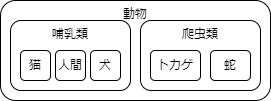
\includegraphics[width=7cm]{./override.png}
  \caption{継承のイメージ}
  \label{inheritance}
\end{figure}

クラスの継承は以下のように行います。
\begin{lstlisting}[caption=クラスの継承,label=inheritance]
class SubClassName(ClassName):
    def __init__(self, arg1, arg2, ...):
        super().__init__(arg1, arg2, ...)
        self.arg1 = arg1
        self.arg2 = arg2
        ...
\end{lstlisting}

\begin{itembox}[l]{\textbf{ポイント}}
  \begin{itemize}
    \item 親クラスのメソッドを呼び出す際はsuper().メソッド名()を使用する
  \end{itemize}
\end{itembox}

猫を基に、子猫クラスを定義してみましょう。
\begin{lstlisting}[caption=子猫クラスの定義,label=kitten]
class Kitten(Cat):
    def __init__(self, name, age, color, mother):
        super().__init__(name, age, color)
        self.mother = mother
    def cry(self):
        print(' にゃーにゃー ')
\end{lstlisting}

子猫クラスは猫クラスを継承しており、cryメソッドをオーバーライドしています。
また、子猫クラスは母猫のオブジェクトを受け取ります。

\section{演習}
メソッドの中身はprint文で何かしらの表示を行うだけでよいです。
\begin{enumerate}
  \item 以下のクラスを定義し、オブジェクトを生成してください。
        \begin{itemize}
          \item クラス名: Dog
          \item 属性: 名前、年齢、毛色
          \item メソッド: bark(吠える)、run(走る)
        \end{itemize}
  \item 以下のクラスを定義し、オブジェクトを生成してください。
        \begin{itemize}
          \item クラス名: Puppy
          \item 親クラス: Dog
          \item 属性: 名前、年齢、毛色、母犬
          \item メソッド: bark(吠える)
        \end{itemize}
  \item 以下のクラスを定義し、オブジェクトを生成してください。
        \begin{itemize}
          \item クラス名: Character
          \item 属性: 名前、HP、MP
          \item メソッド: attack(攻撃)、heal(回復)
        \end{itemize}
  \item 以下のクラスを定義し、オブジェクトを生成してください。
        \begin{itemize}
          \item クラス名: Hero
          \item 親クラス: Character
          \item 属性: 名前、HP、MP、武器
          \item メソッド: attack(攻撃)、heal(回復)
        \end{itemize}
  \item 以下のクラスを定義し、オブジェクトを生成してください。
        \begin{itemize}
          \item クラス名: Slime
          \item 親クラス: Character
          \item 属性: 名前、HP、MP
          \item メソッド: attack(攻撃)、heal(回復)、split(分裂)
        \end{itemize}
\end{enumerate}


\end{document}